\chapter{Diseño e implementación} % Main chapter title

\label{Chapter3} % Change X to a consecutive number; for referencing this chapter elsewhere, use \ref{ChapterX}

En este capítulo se presentan los detalles técnicos de diseño e implementación de la solución IoT que se tuvieron en cuenta durante el desarrollo del trabajo.


\section{Arquitectura de software del sistema}


El sistema cuenta con una arquitectura multi-cloud en la que se integra como hardware el robot de exploración ambiental \citep{cese_gonzalo_memoria} desarrollado en el marco de la Carrera de Especialización en Sistemas Embebidos, con un sistema \textit{back-end} desplegado en la nube de Amazon Web Services \citep{aws}, Smart Contracts desplegados en la red Blockchain Ethereum \cite{ethereum}, y un plataforma analítica de datos desplegada en la nube de Azure \cite{azure} utilizando la herramienta Microsoft Fabric \cite{azure_fabric}. 


En la siguiente figura \ref{fig:software_architecture} podemos apreciar la arquitectura de la solución.


\begin{center}
   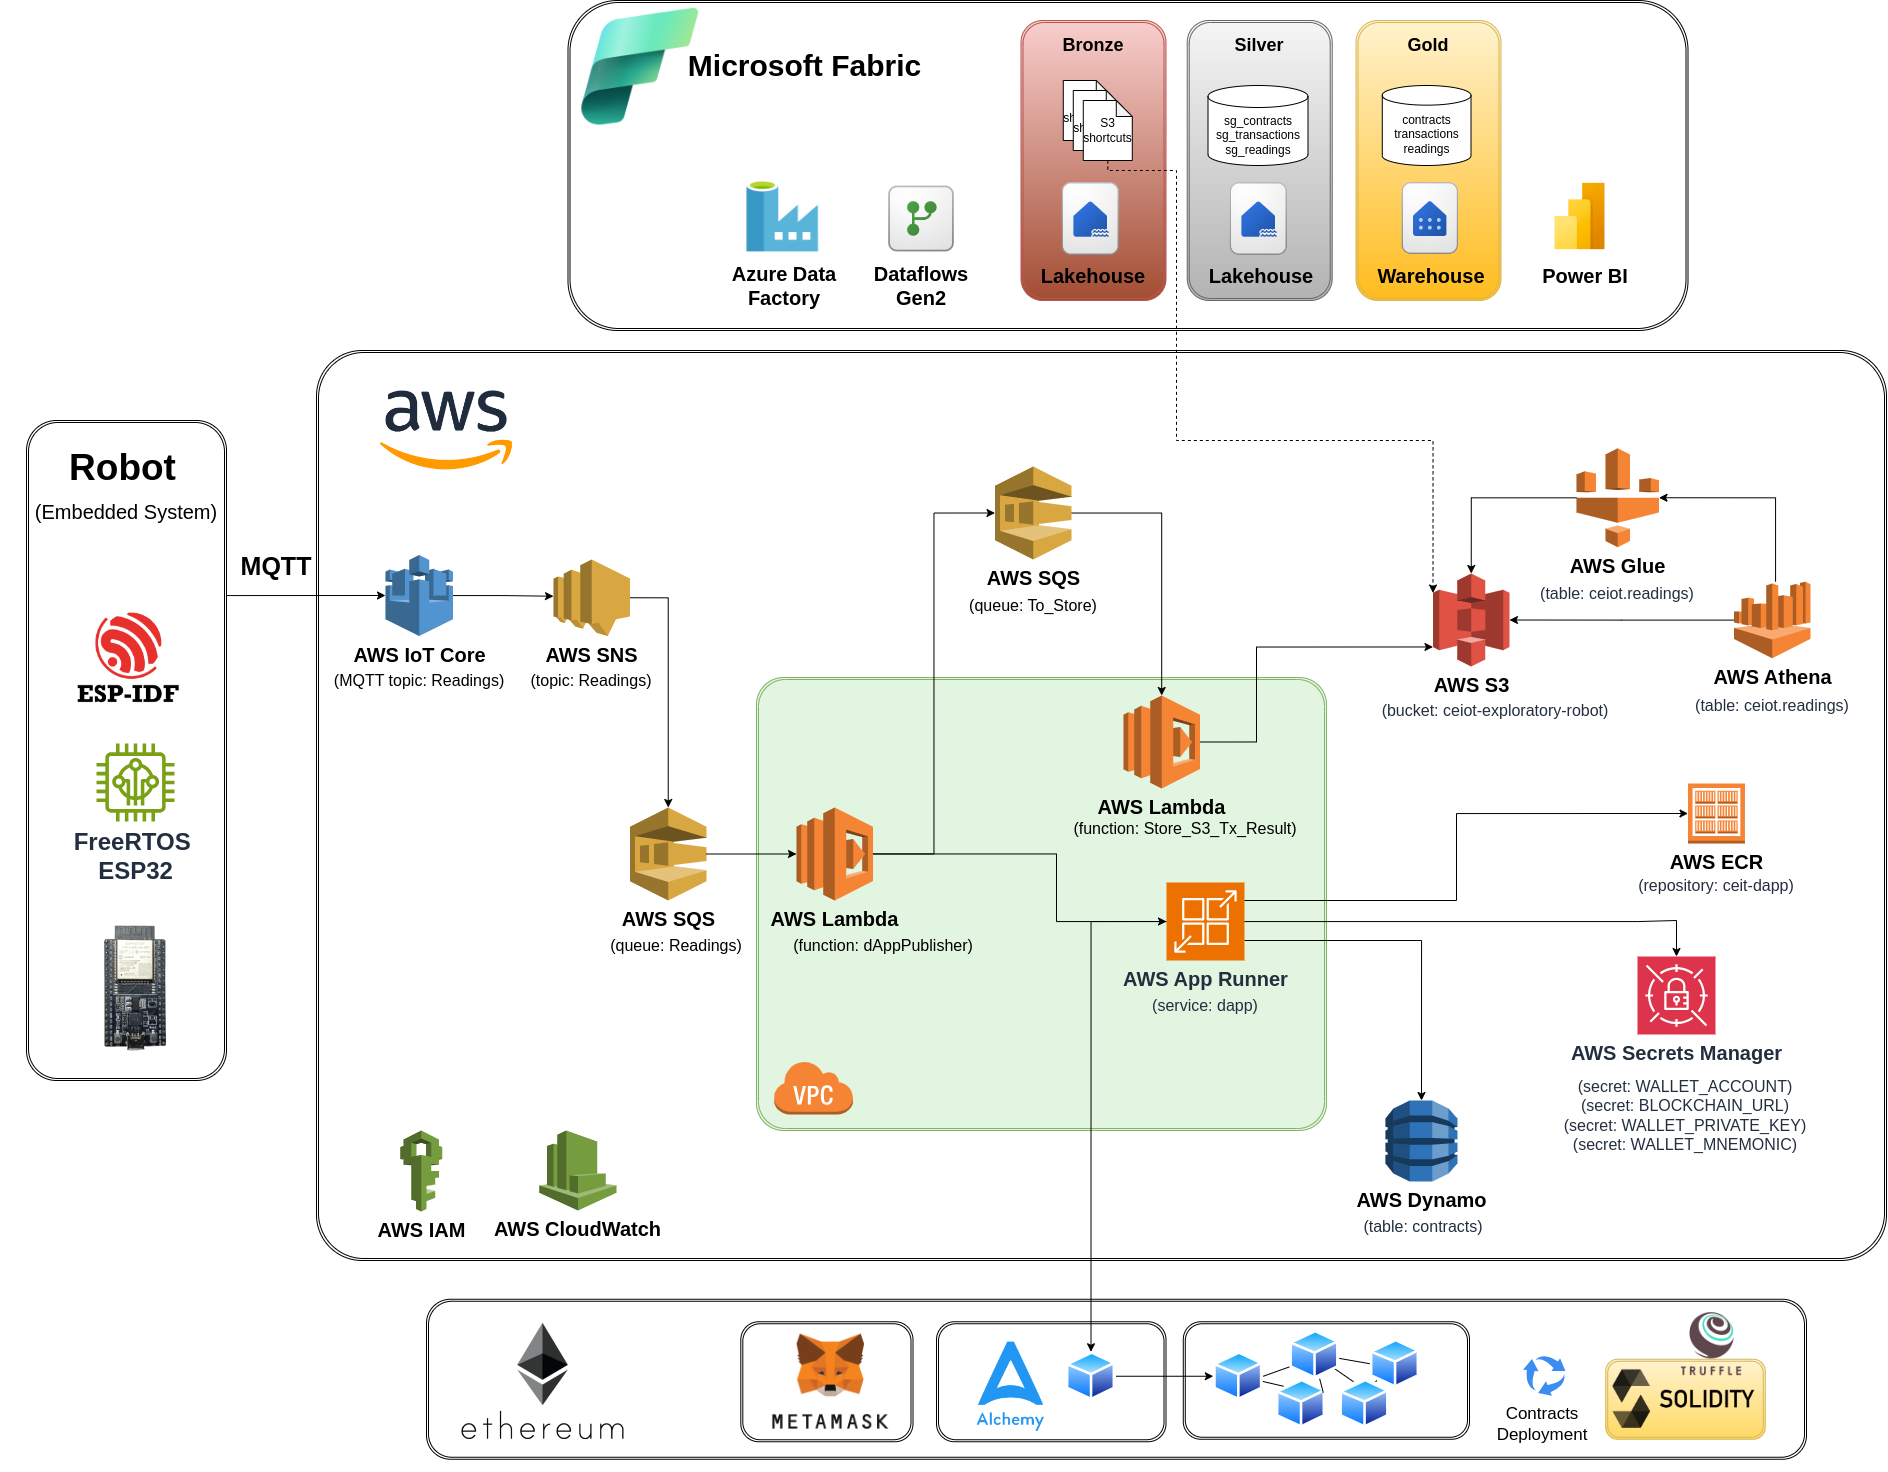
\includegraphics[scale=0.2]{global/software_architecture}
   \captionof{figure}{Arquitectura de la solución.}
   \label{fig:software_architecture}
\end{center}

\section{Hardware e infraestructura del sistema}
 
<A desarrollar>
 
\section{Integración de los módulos y subsistemas}




\subsection{Capa de percepción}


El desarrollo e integración de los componentes de esta capa consistió en la adaptación del firmware desplegado en el robot explorador para extender sus funcionalidades y enviar las lecturas de parámetros ambientales al \textit{topic} MQTT. Dentro de las funcionalidades que se le agregaron al robot explorador se encontraron:

\begin{itemize}
	\item Capturar fecha y hora local del sistema.
	\item Generación de coordenadas geograficas (con datos \textit{mock}).
	\item Conexión segura con tópico MQTT y envío de los datos generados.	
		
\end{itemize}

La configuración de la fecha y hora se realizó por medio del uso del servicio SNTP \citep{sntp} que permite la sincronización del hardware de una red con la fecha y hora provista por servicios externos en estandar en una zona horaria. Esta configuración se realizó incluyendo el encabezado \textbf{esp\_sntp.h} en el código del robot. Una vez realizado esto fue posible obtener la fecha y hora local invocando a la función \textit{localtime}.

La generación de las coordenadas geograficas con datos \textit{mock} se realizo mediante la generación de las ecuaciones \ref{eq:mock_lat} y \ref{eq:mock_long} a continuación.

\begin{equation}
	\label{eq:mock_lat}
	MockLat = \left( \frac{rand()}{RAND\_MAX} \right) \left( LAT\_MAX - LAT\_MIN \right) + LAT\_MIN
\end{equation}
                
\begin{equation}
	\label{eq:mock_long}
	MockLong = \left( \frac{rand()}{RAND\_MAX} \right) \left( LONG\_MAX - LONG\_MIN \right) + LONG\_MIN
\end{equation}

Finalmente, los datos capturados fueron enviados en formato JSON al tópico MQTT con la estructura de la tabla:


\begin{table}[h]
	\centering
	\caption[caption corto]{Tabla de objetos AWS}
	\begin{tabular}{l c c}    
		\toprule
		\textbf{Nombre del campo} & \textbf{Tipo del campo} & \textbf{Descripción}  \\
		\midrule
		deviceId & string & Id del dispositivo \\		
		type & string & Tipo de lectura \\		
		value & string & Valor de la lectura \\		
		geoLat & string & Latitud geográfica \\		
		geoLong & string & Longitud geográfica\\		
		date & string & Fecha \\		
		time & string & Hora \\		
		
		\bottomrule
		\hline
	\end{tabular}
	\label{tab:json_fields}
\end{table}


A continuación podemos apreciar un valor de ejemplo del objeto JSON enviado por el robot:

\begin{lstlisting}
{   	
	"deviceId": "12ad-dao23-ux23",
	"type": "Temperature",
	"value": "0.00",
	"geoLat": "-26.056772",
	"geoLong": "-64.014824",
	"date": "2025-04-1",
	"time": "11:23:59"
}
\end{lstlisting}

\subsection{Capa de red}

El desarrollo de los componentes de esta capa consistió en la publicación de un \textit{topic} MQTT desde el servicio AWS IoT Core y la configuración de la lógica de redirección y almacenamiento de los mensajes recibidos en AWS S3.


Para la conexión segura con el tópico MQTT se configuró el servicio AWS IoT Core, donde se creó una nueva instancia de un dispositivo remoto con el nombre ESP32. Una vez creado este dispositivo se descargaron e instalaron en el código del robot los certificados listados a continuación:


\begin{itemize}
	\item AmazonRootCA1.pem, renombrado a brokerCA.crt:	Es la autoridad certificadora que AWS usa para firmar certificados de sus servidores. El dispositivo lo necesita para verificar la identidad del servidor AWS IoT al conectarse.
	\item dev-certificate.pem.crt, renombrado a client.crt: Contiene la clave pública correspondiente a la clave privada (.key) y está firmado por AWS (o por una CA en la que AWS confía) para verificar la identidad del dispositivo.
	\item dev-private.pem.key, renombrado a client.key: Usada por el dispositivo para firmar su identidad durante la conexión TLS. Nunca se comparte ni se sube a AWS. Tu dispositivo la usa para autenticar su certificado (.crt).
		
\end{itemize}

Una vez realizada la configuración del servicio AWS IoT core e integrado el robot con el tópico, se probó la recepción de lecturas con el cliente de prueba provisto por AWS suscrito al tópico \textit{readings} como puede apreciarse en la figura \ref{fig:aws_iot_core_mqtt_test_2}.


Para el almacenamiento en AWS S3 de los mensajes recibidos, se configuro una \textit{routing rule} o regla de redirección en AWS IoT Core, indicando mediante una consulta con sintaxis SQL, que todos los mensajes recibidos en el tópico \textit{readings} deben almacernarce en el bucket S3 ceiot-exploratory-robot. En la figura \ref{fig:aws_iot_core_message_routing} puede apreciarse esta configuración.
 


Como resultado de la configuración realizada, los mensajes recibidos en MQTT fueron redirigidos y almacenados en AWS S3 como puede apreciarse en la figura \ref{fig:aws_s3_bucket_data2}.



\subsection{Capas de procesamiento y almacenamiento - dApp (AWS) y Smart Contracts}

Uno de los primeros pasos para poder comenzar a desarrollar los componentes blockchain fue la obtención de tokens para poder realizar despliegues y ejecutar la aplicación en las redes de prueba de Ethereum sin utilizar fondos reales. Para Para poder realizar esto, primero fue necesario crear un \textit{wallet} o billetera digital, para lo que se utilizó el servicio Metamask. Luego, para la obtención de créditos se utilizaron los \textit{faucets} de Google \citep{google_faucets}. Como se puede apreciar en las figura \ref{fig:google_faucets2} y tras seleccionar la dirección del \textit{wallet} y \ref{fig:metamask_balance}, tras realizar las transacciones en el \textit{faucet} se reciben los fondos en la billeta digital. 


Posteriormente como podemos apreciar en la figura, en el servicio Etherscan las transacciones realizadas para generar fondos en la dirección de la billetera quedan publicadas en la red.



Una vez obtenidos los fondos de prueba en la billetera se procedió con el desarrollo de los componentes blockchain. Para el desarrollo de los \textit{smart contracts} se utilizó Solidity como lenguaje de programanción y Truffle como herramienta de gestión de configuración, compilación, empaquetado y despliegue. Truffle utiliza una configuración basada en archivos Javascript para la descripción de las tareas, y para realizar el despliegue a diferentes redes, como por ejemplo de forma local a Ganache o de forma remota a redes como Sepolia, Holesky y Mainnet. En la los archivos de configuración de Truffle se agregaron entradas para poder desplegar a Ganache y a Sepolia como se puede apreciar en la figura \ref{fig:truffle_redes}.

\begin{center}
   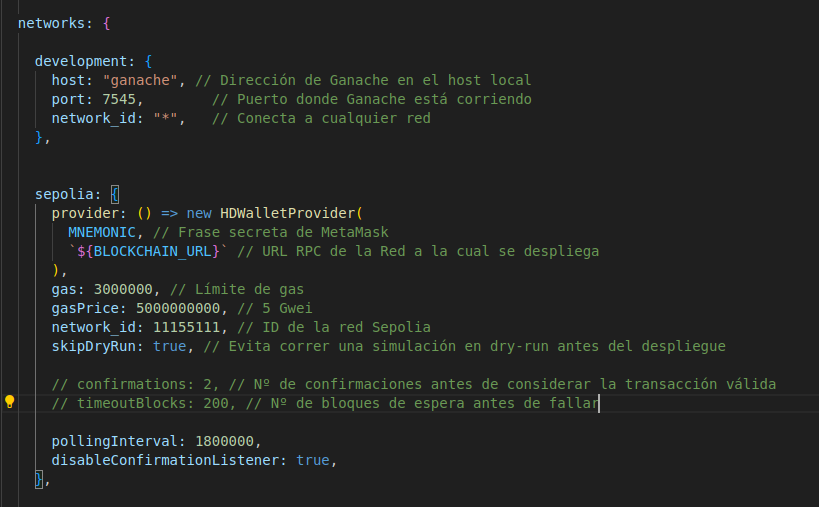
\includegraphics[scale=0.4]{blockchain/truffle_redes}
   \captionof{figure}{Configuración de redes de despliegue en Truffle.}
   \label{fig:truffle_redes}
\end{center}

Como se puede apreciar en la figura \ref{fig:sm_deployment}, durante el proceso de despliegue se presenta cierta información por pantalla:

\begin{itemize}
	\item La red a la cual se esta realizando el despliegue.
	\item Los \textit{smart contracts} incluidos en el despliegue y la dirección que toman una vez desplegados. 
	\item El \textit{hash} o identificador de la transacción.
	\item El número de bloque en el que se encuentra la transacción de despliegue.
	\item La dirección de la billetera digital y el balance disponible previo a la transacción.
	\item La cantidad de gas utilizado en el despliegue, el costo unitario y el costo total de la transacción.
\end{itemize}

Luego de haber realizado el despliegue de los \textit{smart contracts} a la red Sepolia, se puede evidenciar desde Etherscan las transacciones reportadas en la salida por pantalla (figura \ref{fig:sm_deployment_etherscan1}) y comparar los valores. Como se puede apreciar en la figura \ref{fig:sm_deployment_etherscan2}, al ingresar a los detalles de la transacción podemos obtener mas información del contrato.


Desde el punto de vista del \textit{backend} blockchain, se desarrolló la dApp utilizando Node.js y la biblioteca Javascript Web3.js para la comunicación con los \textit{smart contracts}. Para la dApp, se desarrollaron varios \textit{endpoints} y se expusieron mediante el estandar Open API \citep{open_api} utilizando la biblioteca Swagger, que como se puede apreciar en la figura \ref{fig:dapp_endpoints}, genera una interfaz gráfica documenta y brinda un cliente de prueba para poder invocar los \textit{endpoints} expuestos.


Para que la dApp pueda interactuar con la red debe poder conectarse a un endpoint RPC publicado desde cualquier nodo de la misma. Por este motivo se utilizó el servicio Alchemy que brinda publica endpoints para distintas redes, incluyendo Ethereum. Primero se creó un perfil en este servicio de manera gratuita y se creó un nuevo proyecto con el nombre iot\_robots\_storage. Una vez hecho esto se pudo acceder a los diferentes endpoints disponibles de Ethereum para las tres redes principales (Mainnet, Holesky y Sepolia) como se puede apreciar en la figura \ref{fig:alchemy1}. Posteriormente, se configuró en la inicialización de la biblioteca Web3.js en la dApp, el endpoint provisto por Alchemy y el app\_key del proyecto iot\_robots\_storage. 

La dApp fue desplegada utilizando el servicio AWS App Runner por medio de la creación y publicación en AWS ECR de una imagen Docker con el código de la misma. Se configuró el despliegue de la dApp para que se encuentre en una VPC (red privada) con reglas que impiden el tráfico HTTP de ingreso desde la red pública, pero permiten el tráfico saliente, de esta manera la dApp puede acceder al servicio Alchemy e invocar los \textit{Smart Contracts}.

Además de la URL y el key del proyecto en Alchemy, la dApp necesita ciertos datos sensibles para poder acceder a Ethereum, firmar transacciones, y realizar escrituras (ya que dichas operaciones requieren el pago de un fee). Estos datos al ser considerados sensibles, fueron almacenados en el servicio AWS Secret Manager, y accedidos a través del uso de su integración en los diferentes componentes. En la siguiente lista se pueden apreciar el propósito de los mismos:

\begin{itemize}
	\item Wallet Account: identificador unívoco de una cuenta en la red de blockchain.
	\item Wallet Mnemonic: conjunto de entre 12 y 24 palabras que forman la semilla criptográfica para acceder (o recuperar la cuenta) y generar claves privadas, entre otras cosas.
	\item Wallet Private Key: Es generado mediante el Mnemonic, y es necesario para firmar transacciones de escritura.
\end{itemize}


\subsection{Capas de distribución de eventos}


Una vez configurados servicios AWS IoT Core y AWS AppRunner se procedió al despliegue de los componentes que permiten la distribución asíncrona de eventos desde el flujo de ingesta en tiempo real MQTT al posterior almacenamiento en blockchain de las lecturas y en S3 de los resultados de dichas transacciones. Para esto se configuraron los servicios AWS SNS y SQS para brindar, por medio de SNS, una interfaz pub/sub que permita la distribución en paralelo de los eventos recibidos a los topicos suscriptos, y por medio de SQS, un encolamiento de eventos para cada suscriptor de forma que se pueda paralelizar el procesamiento de los eventos.

Dentro de la misma VPC donde se encuentra la dApp (en AWS App Runner) se desplegaron dos funcionas AWS Lambda para la integración entre el flujo de lecturas ambientales, la dApp y el almacenamiento S3:

\begin{itemize}
	\item Send Reading to Blockchain (Python): Implementa la lógica para recibir eventos provenientes de SQS, y construir el request que la dApp espera para poder invocar al Smart Contract pasando los datos como parámetros. Al invocar a la dApp espera la confirmación de la transacción en blockchain y cuando recibe la respuesta la envia a la cola ToStore para ser escrita en S3.
	\item Write Readings and Transactions (Python): Recibe de la cola ToStore la lectura y transacción confirmada, y posteriormente almacena ambos objetos en S3.
\end{itemize}

Desde el punto de vista de infraestructura, como AWS Lambda hace uso de los servicios SQS y S3, que se encuentran expuestos a la red pública, se configuraron AWS Endpoints para integrar la VPC con S3 y SQS de manera interna (sin pasar por la red pública).


\subsection{Capas de procesamiento y almacenamiento de datos}

Una vez realizadas las configuraciones de ingesta de datos en \textit{streaming} se realizaron las configuraciones para poder accederlos, administrarlos y procesarlos de forma batch.
Para ello se crearon una base de datos y una tabla en AWS Glue para representar el esquema de datos almacenados en AWS S3 en formato JSON, como se puede apreciar en la figura \ref{fig:aws_glue_table_review}.

\begin{center}
   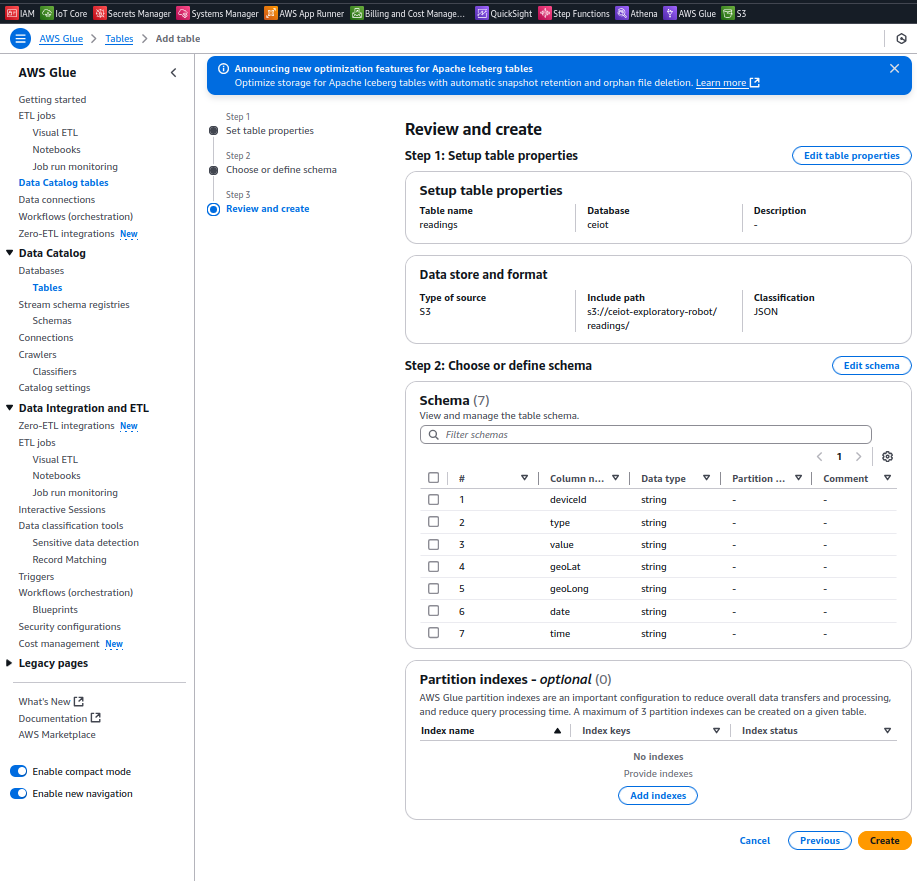
\includegraphics[scale=0.4]{AWS/aws_glue_table_review}
   \captionof{figure}{Creación de base datos, tabla y esquema AWS Glue.}
   \label{fig:aws_glue_table_review}
\end{center}

Con el esquema de datos definido en el catálogo de AWS Glue, fue posible realizar consultas SQL sobre los datos almacenados en AWS S3 desde AWS Athena, como se puede apreciar en la figura 

Para la capa de ingeniería de datos, procesamiento de analíticas y creación de reportes y dashboards, se decidió utilizar la suite de componentes provista por Microsoft Fabric en la nube de Azure.
El diseño de la solución de datos implementada se basó en la arquitectura Medallion donde se implementaron las tres capas estándares (Bronze, Silver y Gold), y se almacenaron los datos en el Data Lake OneLake en formato Delta. La separación en capas se realizó de la siguiente manera:

\begin{itemize}
	\item Capa Bronze: se integró el Fabric Lakehouse con el almacenamiento S3 mediante la configuración de \textit{shortcuts}. Los datos se encontraron almacenados en crudo y con formato JSON.
	\item Capa Silver: se almacenaron y accedieron en el Fabric Lakehouse las tres diferentes entidades (contracts, transactions y readings) en formato de tablas Delta (con archivos Parquet), utilizando el lenguaje SQL a través del SQL Endpoint provisto por Lakehouse. En esta capa los datos se encuentran en estado \textit{staging} en el cual sufren transformaciónes y enrriquecimiento para mejorar su calidad.
	\item Capa Gold: se almacenaron y accedieron el el Fabric Warehouse las tres diferentes entidades (contracts, transactions y readings) como tablas de un modelo relacional SQL. En esta capa los datos se encuentran en su calidad final listos para poder ser entregados y consumidos desde herramientas de visualización y reportes.
\end{itemize}

El proceso de transformación de datos utilizado se baso principalmente en el uso de las herramientas Azure Data Factory y Dataflows Gen2. Con Azure Data Factory se diseñó la orquestación del procesamiento de datos y se utilizaron actividades de copiado y transformación de datos. En la siguiente figura \ref{fig:datafactory_pipeline} puede apreciarse el \textit{data pipeline} en Azure Data Factory:

\begin{center}
   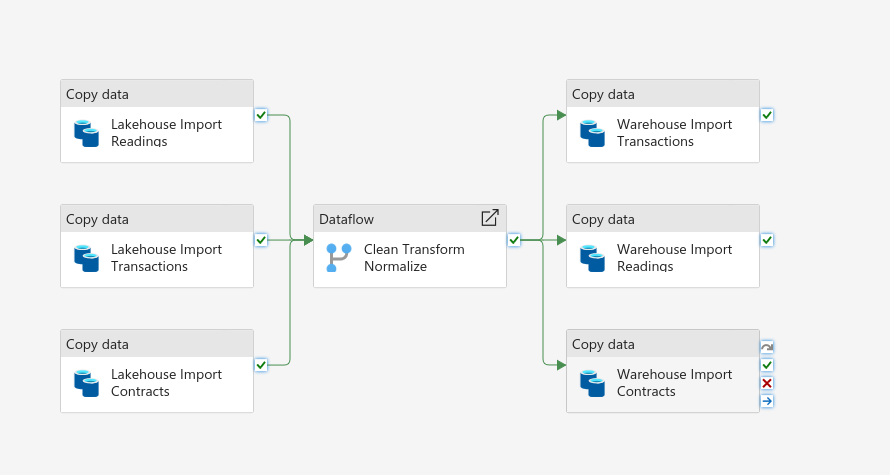
\includegraphics[scale=0.4]{Azure/datafactory_pipeline}
   \captionof{figure}{Azure Data Factory pipeline.}
   \label{fig:datafactory_pipeline}
\end{center}

El flujo esta estructurado de la siguiente manera:
\begin{itemize}

	\item Las tres primeras actividades de movimiento de datos tienen como propósito la copia de datos desde AWS S3 a Fabric OneLake, tranformando el formato de JSON crudo sin compresion a archivos Parquet con compresion Snappy (un 30 por ciento del tamanio original), con la generación y validación del esquema de datos al ser importado como tabla Delta dentro del LakeHouse. Esta actividad se realiza para las tres entidades (contracts, transactions, y readings).
	
	\item La siguiente actividad es la transformación y curado de los datos usando Dataflows Gen2. Los detalles de la misma se explican mas abajo.
	
	\item Finalmente, las ultimas tres actividades son el movimiento de los datos curados en el Lakehouse a la capa Gold en el Warehouse, donde ya se encuentran listos para ser utilizados en el Semantic Model de PowerBI.
\end{itemize}

Para la transformación y limpieza de datos se instanció el componente Dataflows Gen2 desde Azure Data Factory. Posteriormente desde la interfaz de la herramienta Dataflows se configuraron las diferentes actividades de transformación y curado de datos para cada una de las entidades procesadas. En la siguiente figura \ref{fig:dataflows_pipeline} podemos apreciar la orquestasción de estas transformaciones desde Dataflows:

\begin{center}
   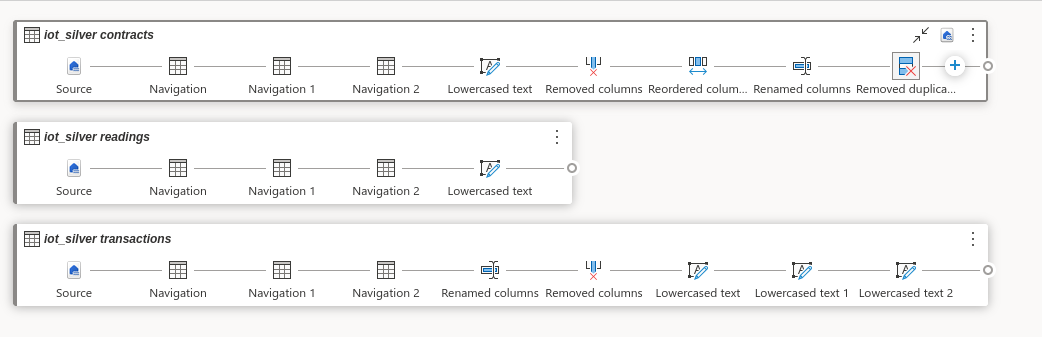
\includegraphics[scale=0.4]{Azure/dataflows_pipeline}
   \captionof{figure}{Dataflows pipeline.}
   \label{fig:dataflows_pipeline}
\end{center}

Como podemos apreciar se aplican diferentes transformaciones dependiendo de la entidad. Las transformaciones realizadas fueron la transformación de los datos a lowercase para algunas columnas con el fin de poder ser cruzadas adecuadamente con las otras entidades, la eliminaación ciertas columnas innecesarias que solo consumen espacio y no resultan de interés para los reportes finales, el reordenamiento de las columnas para la presentación final, y el renombrado  de algunas columnas para estandarizar el acceso.
	
Una vez en el data Warehouse en su capa Gold se creó un Semantic Model de Power BI para poder representar los datos en los reportes. Luego se establecieron las relaciones entre las tres entidades y se crearon ciertas métricas adicionales en para poder facilitar el cálculo dinámico de valores en los dashboards. En la siguiente figura \ref{fig:semantic_model} podemos apreciar una imagen del mismo:

\begin{center}
   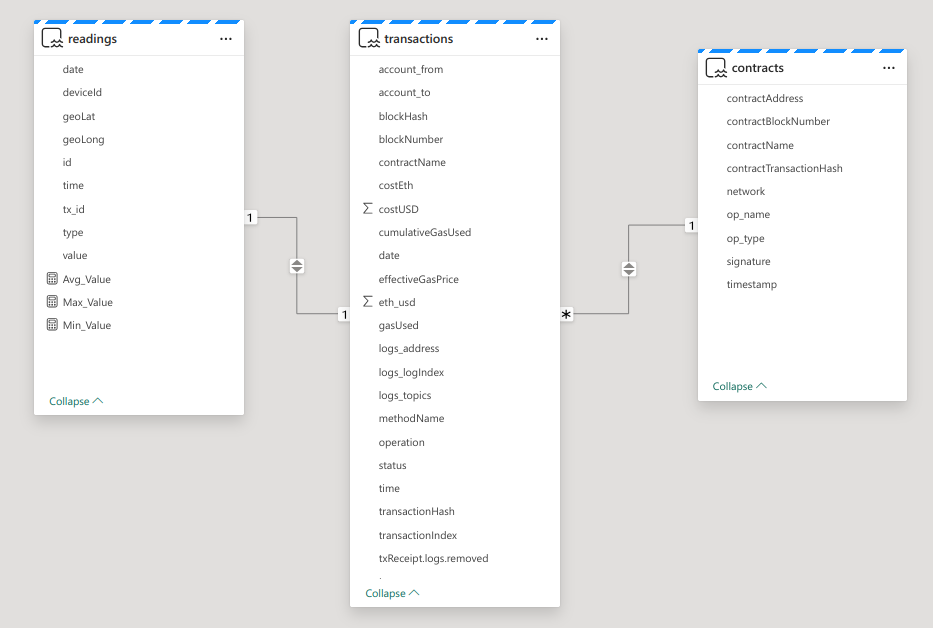
\includegraphics[scale=0.3]{Azure/semantic_model}
   \captionof{figure}{Modelo semántico de PowerBI.}
   \label{fig:semantic_model}
\end{center}

Las métricas creadas fueron:

\begin{itemize}
	\item Readings - Avg Value (valor promedio)
	\item Readings - Max Value (valor máximo)
	\item Readings - Min Value (valor mínimo)
\end{itemize}

Finalmente desde PowerBI se construyeron los reportes compuestos por tablas dinámicas y graficos. Como los datos fueron relacionados en el Semantic Model, al seleccionar valores en el reporte se realiza dinamicamente un filtrado lo cual permite el análisis de la información para la toma de decisiones. En la siguientes figuras \ref{fig:powerbi1} podemos apreciar algunas capturas de algunos de los dashboards generados:



\section{Plataforma de desarrollo y despliegue}



\section{Tabla de todos los objetos cloud creados}




\begin{table}[h]
	\centering
	\caption[caption corto]{Tabla de objetos AWS}
	\begin{tabular}{l c c}    
		\toprule
		\textbf{Servicio} & \textbf{Propósito} & \textbf{Nombre de objeto}  \\
		\midrule
		AWS IoT Core & \textit{Thing} & ESP32 \\		
		AWS IoT Core & \textit{MQTT topic} & readings \\		
		AWS IoT Core & \textit{Routing Rule} & StoreToS3 \\		
		AWS S3 & Bucket & ceiot-exploratory-robot \\	
		AWS Glue & \textit Base de datos & ceit \\		
		AWS Glue & Tabla & \textit{Readings} \\		

		\bottomrule
		\hline
	\end{tabular}
	\label{tab:peces}
\end{table}

